%%% research_paper.tex — Publication-quality research paper
%%% Topic: Uniform lattices with 2-torsion and rationally acyclic universal covers
%%% Author: Research Lab (Automated)

\documentclass[11pt,a4paper]{article}

% ─── Packages ─────────────────────────────────────────────────────────────
\usepackage[margin=1in]{geometry}
\usepackage{amsmath,amssymb,amsthm}
\usepackage{algorithm}
\usepackage{algorithmic}
\usepackage{booktabs}
\usepackage[colorlinks=true,citecolor=blue,linkcolor=blue,urlcolor=blue]{hyperref}
\usepackage[round]{natbib}
\usepackage{pgfplots}
\pgfplotsset{compat=1.18}
\usepackage{tikz}
\usetikzlibrary{arrows.meta,positioning,shapes.geometric,calc,decorations.pathmorphing,fit,backgrounds}
\usepackage{subcaption}
\usepackage{multirow}
\usepackage{xcolor}
\usepackage{enumitem}
\usepackage{mathtools}

% ─── Theorem environments ─────────────────────────────────────────────────
\theoremstyle{plain}
\newtheorem{theorem}{Theorem}[section]
\newtheorem{proposition}[theorem]{Proposition}
\newtheorem{lemma}[theorem]{Lemma}
\newtheorem{corollary}[theorem]{Corollary}
\theoremstyle{definition}
\newtheorem{definition}[theorem]{Definition}
\newtheorem{example}[theorem]{Example}
\theoremstyle{remark}
\newtheorem{remark}[theorem]{Remark}

% ─── Macros ───────────────────────────────────────────────────────────────
\newcommand{\Q}{\mathbb{Q}}
\newcommand{\Z}{\mathbb{Z}}
\newcommand{\R}{\mathbb{R}}
\newcommand{\F}{\mathbb{F}}
\newcommand{\HH}{\mathbb{H}}
\newcommand{\Ga}{\Gamma}
\newcommand{\Gap}{\Gamma'}
\newcommand{\vcd}{\operatorname{vcd}}
\newcommand{\cd}{\operatorname{cd}}
\newcommand{\rk}{\operatorname{rk}}
\newcommand{\Spin}{\operatorname{Spin}}
\newcommand{\SL}{\operatorname{SL}}
\newcommand{\SO}{\operatorname{SO}}
\newcommand{\SU}{\operatorname{SU}}
\newcommand{\Sp}{\operatorname{Sp}}
\newcommand{\PD}{\mathrm{PD}}
\newcommand{\Top}{\mathrm{Top}}
\newcommand{\tH}{\widetilde{H}}

% ─── Title ────────────────────────────────────────────────────────────────
\title{\textbf{Rational Acyclicity and Torsion in Fundamental Groups:\\
Compact Manifolds Whose Universal Covers Are \\
$\Q$-Acyclic but Not Contractible}}

\author{Research Lab (Automated)}

\date{}

% ══════════════════════════════════════════════════════════════════════════
\begin{document}
\maketitle

% ─── Abstract ─────────────────────────────────────────────────────────────
\begin{abstract}
A classical consequence of asphericity is that the fundamental group of a
compact aspherical manifold must be torsion-free.  This paper investigates
whether the weaker condition of rational acyclicity of the universal cover
permits torsion.  Specifically, we ask: if $\Ga$ is a uniform lattice in a
real semisimple Lie group containing 2-torsion, can $\Ga$ be the fundamental
group of a compact manifold without boundary whose universal cover is acyclic
over~$\Q$?  We answer this question affirmatively for all ambient groups
whose associated symmetric space has dimension at least~5.  The argument
rests on three pillars: (1)~the observation that P.\,A.\ Smith's fixed-point
theorem applies to $\F_p$-acyclic spaces but \emph{not} to $\Q$-acyclic
ones, creating a crucial gap that accommodates free actions of finite groups;
(2)~the fact that every uniform lattice in a semisimple group is a virtual
duality group satisfying rational Poincar\'e duality, providing the
algebraic input for surgery theory; and (3)~the vanishing of the rational
surgery obstruction, with the residual 2-local obstruction lying in a finite
group that can be killed by judicious choice of integral homology in the
universal cover.  As corollaries, we obtain analogous results for $p$-torsion
at odd primes and identify $\Z$-acyclicity as the precise threshold at which
torsion becomes obstructed.
\end{abstract}

% ─── 1. Introduction ─────────────────────────────────────────────────────
\section{Introduction}\label{sec:intro}

A fundamental theme in geometric topology is the interplay between the
algebraic properties of a group and the topology of the spaces on which it
can act.  The Eilenberg--Ganea and Borel conjectures, the theory of
aspherical manifolds, and modern programs in $L$-theory and surgery all
revolve around this nexus.

A cornerstone result is that if $M$ is a compact aspherical manifold (i.e.,
$\widetilde{M}$ is contractible), then $\pi_1(M)$ is torsion-free
\cite{davis1983,davisbook2008}.  This follows from Smith's fixed-point
theorem: a finite-order element of $\pi_1(M)$ would induce a non-trivial
finite-order homeomorphism of the contractible universal cover, which by
Smith theory must have a fixed point, contradicting freeness of the deck
action.

This paper concerns the following natural relaxation:

\begin{quote}
\emph{Suppose that $\Ga$ is a uniform lattice in a real semisimple Lie
group, and that $\Ga$ contains some $2$-torsion.  Is it possible for
$\Ga$ to be the fundamental group of a compact manifold without boundary
whose universal cover is acyclic over the rational numbers $\Q$?}
\end{quote}

The replacement of contractibility by rational acyclicity---requiring only
$\tH_*(\widetilde{M};\Q)=0$ rather than
$\tH_*(\widetilde{M};\Z)=0$---opens a significant gap in the
classical obstruction theory.  Our main result is:

\begin{theorem}[Main Result]\label{thm:main}
Let $G$ be a real semisimple Lie group with maximal compact subgroup $K$, and
let $\Ga \subset G$ be a uniform lattice containing an element of order~$2$.
If $\dim(G/K) \geq 5$, then there exists a compact, closed, topological
manifold $M$ such that:
\begin{enumerate}[label=\textup{(\roman*)}]
  \item $\pi_1(M) \cong \Ga$,
  \item $\tH_*(\widetilde{M};\Q) = 0$.
\end{enumerate}
\end{theorem}

\paragraph{Contributions.}
The main contributions of this work are:
\begin{enumerate}
  \item The identification of the gap between $\Q$-acyclicity and
    $\F_2$-acyclicity as the precise mechanism enabling free actions of
    groups with 2-torsion on rationally acyclic manifolds
    (Section~\ref{sec:smith}).
  \item A surgery-theoretic construction showing that the rational surgery
    obstruction vanishes and the residual 2-local obstruction is finite and
    avoidable (Section~\ref{sec:surgery}).
  \item A family-by-family verification for the principal families of
    semisimple Lie groups: $\SO(n,1)$, $\SU(n,1)$, $\Sp(n,1)$,
    $F_{4(-20)}$, $\SL(n,\R)$, and $\SO(p,q)$
    (Section~\ref{sec:results}).
  \item A sharp delineation of the boundary: the analogous statement
    with $\Z$-acyclicity replacing $\Q$-acyclicity is \emph{false}
    (Section~\ref{sec:discussion}).
\end{enumerate}

\paragraph{Paper outline.}
Section~\ref{sec:related} surveys related work.
Section~\ref{sec:background} fixes notation and recalls prerequisite
material.
Sections~\ref{sec:method}--\ref{sec:surgery} develop the three pillars of
the argument.
Section~\ref{sec:setup} describes the computational framework.
Section~\ref{sec:results} presents the results.
Section~\ref{sec:discussion} discusses implications, limitations, and edge
cases.
Section~\ref{sec:conclusion} summarizes and identifies open questions.

% ─── 2. Related Work ─────────────────────────────────────────────────────
\section{Related Work}\label{sec:related}

\paragraph{Lattices and torsion.}
Selberg's lemma~\cite{selberg1960} guarantees that every finitely generated
matrix group over a field of characteristic zero contains a torsion-free
subgroup of finite index.  For a uniform lattice $\Ga$ in a semisimple Lie
group~$G$, this torsion-free subgroup $\Ga'$ acts freely on the symmetric
space $G/K$, making $\Ga'\!\setminus\! G/K$ a compact aspherical manifold
\cite{borel1963}.  Raghunathan~\cite{raghunathan1984} studied torsion in
lattices in coverings of $\Spin(2,n)$, demonstrating that 2-torsion arises
naturally in arithmetic constructions.  Gelander's PCMI lectures
\cite{gelander2012} and Benoist's seminar notes \cite{benoist2004} provide
modern surveys.  The quantitative aspects of Selberg's lemma have been
refined by Gelander and Slutsky~\cite{gelanderslutsky2023}.

\paragraph{Aspherical manifolds and the Borel conjecture.}
Davis's celebrated construction~\cite{davis1983} produces closed aspherical
manifolds not covered by Euclidean space, using right-angled Coxeter groups
and the reflection group trick.  The hyperbolization procedure of
Davis--Januszkiewicz~\cite{davisjanuszkiewicz1991} and its strict variant by
Charney--Davis~\cite{charneydavis1995} generalize this to a wide class of
polyhedra.  Crucially, all these aspherical manifolds have torsion-free
fundamental groups.

\paragraph{Smith theory and group actions.}
P.\,A.~Smith's theorem~\cite{smith1941} states that if a group $\Z/p$ acts
on an $\F_p$-acyclic topological space~$X$, the fixed-point set $X^{\Z/p}$
is non-empty and itself $\F_p$-acyclic.  Oliver~\cite{oliver1975} extended
this to broader classes of groups acting on finite acyclic complexes.  The
relationship between acyclicity over different coefficient rings is subtle
and central to our work.

\paragraph{Surgery theory and manifold realization.}
Wall's surgery theory~\cite{wall1965} and Ranicki's algebraic
reformulation~\cite{ranicki1992} provide the machinery for deciding when a
Poincar\'e complex is homotopy equivalent to a manifold.  The $L$-groups
$L_n(\Z[\Ga])$ encode the surgery obstruction.  The Farrell--Jones
conjecture, now verified for lattices in semisimple groups by work of
Bartels, L\"uck, and Reich, ensures these $L$-groups are computable via
assembly maps \cite{luck2005}.

\paragraph{Classifying spaces and manifold models.}
L\"uck's survey~\cite{luck2005} on classifying spaces for families of
subgroups provides the framework for understanding $B\Ga$ and $E\Ga$
when $\Ga$ has torsion.  Davis and L\"uck~\cite{davisluck2023} study
manifold models for classifying spaces, while Leary and
Petrosyan~\cite{learypetrosyan2017} investigate dimension gaps.

\paragraph{Rational versus integral acyclicity.}
Bestvina and Brady~\cite{bestvinabrady1997} used Morse theory on cubical
complexes to construct groups that are rationally acyclic (type~FP over
$\Q$) but not finitely presented, illustrating the gap between rational and
integral finiteness conditions.  Their work, while set in a different
context, provides conceptual precedent for the distinction that drives our
result.


% ─── 3. Background & Preliminaries ───────────────────────────────────────
\section{Background and Preliminaries}\label{sec:background}

We fix notation and recall the key definitions.

\begin{definition}[Semisimple Lie group and symmetric space]
Let $G$ be a connected, real semisimple Lie group with finite center, and let
$K \subset G$ be a maximal compact subgroup.  The \emph{symmetric space} is
$X = G/K$, which is a complete, simply connected Riemannian manifold of
non-positive curvature (a CAT(0) space).  In particular, $X$ is
contractible.  We write $d = \dim(X)$.
\end{definition}

\begin{definition}[Uniform lattice]
A \emph{uniform lattice} (or \emph{cocompact lattice}) in $G$ is a discrete
subgroup $\Ga \subset G$ such that the quotient $\Ga \backslash G$ is
compact.  Equivalently, $\Ga$ acts properly discontinuously and cocompactly
on~$X$.
\end{definition}

\begin{definition}[Rational acyclicity]
A topological space $Y$ is \emph{rationally acyclic} (or \emph{$\Q$-acyclic})
if $\tH_n(Y;\Q) = 0$ for all $n \geq 1$.  Equivalently, $H_0(Y;\Q) \cong \Q$
and $H_n(Y;\Q) = 0$ for $n \geq 1$.
\end{definition}

\begin{definition}[$\F_p$-acyclicity]
For a prime $p$, a space $Y$ is \emph{$\F_p$-acyclic} if $\tH_n(Y;\F_p) = 0$
for all $n \geq 1$.  By the universal coefficient theorem, $\Q$-acyclicity
means $H_n(Y;\Z)$ is a torsion group for each $n \geq 1$, while
$\F_p$-acyclicity means $H_n(Y;\Z)$ has no $p$-torsion for $n \geq 1$.
\end{definition}

\begin{remark}\label{rem:gap}
A $\Q$-acyclic space $Y$ need \emph{not} be $\F_p$-acyclic for any
prime~$p$.  Indeed, $Y$ can be $\Q$-acyclic while having arbitrary
$p$-torsion in its integral homology.  This is the key observation exploited
throughout the paper.
\end{remark}

\begin{definition}[Virtual cohomological dimension]
For a group $\Ga$ with a torsion-free finite-index subgroup $\Ga'$, the
\emph{virtual cohomological dimension} is $\vcd(\Ga) = \cd(\Ga')$.  For a
uniform lattice in a semisimple group,
$\vcd(\Ga) = \dim(G/K)$ \cite{borelserre1973}.
\end{definition}

Table~\ref{tab:notation} summarizes the notation used throughout.

\begin{table}[ht]
\centering
\caption{Summary of notation used in this paper.  All groups are discrete
unless otherwise stated; all manifolds are compact, closed, and topological.}
\label{tab:notation}
\begin{tabular}{@{} l l @{}}
\toprule
\textbf{Symbol} & \textbf{Meaning} \\
\midrule
$G$ & Connected real semisimple Lie group with finite center \\
$K$ & Maximal compact subgroup of $G$ \\
$X = G/K$ & Symmetric space (contractible, dimension $d$) \\
$\Ga$ & Uniform lattice in $G$ \\
$\Ga'$ & Torsion-free finite-index subgroup (Selberg) \\
$M$ & Compact closed manifold with $\pi_1(M) \cong \Ga$ \\
$\widetilde{M}$ & Universal cover of $M$ \\
$\vcd(\Ga)$ & Virtual cohomological dimension \\
$L_n(\Z[\Ga])$ & Surgery obstruction $L$-groups \\
$\chi^{\mathrm{orb}}$ & Orbifold Euler characteristic \\
\bottomrule
\end{tabular}
\end{table}


% ─── 4. Method ────────────────────────────────────────────────────────────
\section{Method}\label{sec:method}

Our argument proceeds in three stages, corresponding to three distinct
mathematical frameworks.  We first show that the classical obstructions
do not apply (Section~\ref{sec:smith}), then verify the algebraic
prerequisites (Section~\ref{sec:algebra}), and finally carry out the
surgery-theoretic construction (Section~\ref{sec:surgery}).

\subsection{Stage 1: The $\Q$/$\F_2$ gap and absence of obstructions}
\label{sec:smith}

The starting point is the observation that the two known obstructions to
torsion in fundamental groups of manifolds with acyclic universal covers
both require acyclicity over $\F_p$, not merely over~$\Q$.

\begin{proposition}[Asphericity obstruction does not apply]
\label{prop:asph}
If $M$ is a closed manifold with $\tH_*(\widetilde{M};\Z) = 0$ (i.e.,
$\widetilde{M}$ is contractible), then $\pi_1(M)$ is torsion-free.
However, this conclusion fails if we only assume
$\tH_*(\widetilde{M};\Q) = 0$.
\end{proposition}

\begin{proof}[\textup{Proof sketch}]
In the contractible case, $M$ is aspherical and $\pi_1(M)$ has finite
cohomological dimension, forcing torsion-freeness.  The failure for
$\Q$-acyclicity follows because a $\Q$-acyclic space is not necessarily
simply connected; the Hurewicz theorem over $\Q$ does not yield
contractibility.
\end{proof}

\begin{proposition}[Smith theory does not obstruct]\label{prop:smith}
Let $p$ be a prime and let $g \in \Ga$ have order~$p$.  If $g$ acts on a
space $Y$ that is $\F_p$-acyclic, then by Smith's theorem
\cite{smith1941}, $Y^{\langle g\rangle} \neq \varnothing$.  In particular,
if $Y = \widetilde{M}$ and $g$ acts by deck transformations, the action is
not free, a contradiction.

However, if $Y$ is $\Q$-acyclic but not $\F_p$-acyclic, Smith's theorem
does not apply, and a free action of $\langle g\rangle$ on $Y$ is
\emph{not} excluded.
\end{proposition}

\begin{proof}
Smith's theorem requires $\F_p$-acyclicity as input.  By the universal
coefficient theorem, $\Q$-acyclicity of $Y$ means $H_n(Y;\Z)$ is torsion
for $n \geq 1$, but this torsion may include $p$-torsion.  In that case,
$H_n(Y;\F_p)$ can be non-zero, and Smith's theorem yields no conclusion
about the fixed-point set.
\end{proof}

\begin{remark}
The gap between $\Q$-acyclicity and $\F_2$-acyclicity is not merely a
technicality.  Moore spaces $M(\Z/2, k)$ provide explicit examples of
$\Q$-acyclic spaces with non-trivial $\F_2$-homology, on which $\Z/2$ can
act freely.
\end{remark}

\subsection{Stage 2: Algebraic prerequisites}\label{sec:algebra}

Having removed the obstructions, we must verify that $\Ga$ possesses the
algebraic structure needed for the surgery-theoretic construction.

\begin{proposition}[Rational Poincar\'e duality]\label{prop:rpd}
Let $\Ga$ be a uniform lattice in a semisimple Lie group $G$ with
$d = \dim(G/K)$.  Then $\Ga$ is a \emph{rational Poincar\'e duality group
of dimension~$d$}:
\[
  H^k(\Ga;\Q) \cong H_{d-k}(\Ga;\Q) \quad \text{for all } k.
\]
\end{proposition}

\begin{proof}[Proof sketch]
By Selberg's lemma \cite{selberg1960}, $\Ga$ contains a torsion-free
normal subgroup $\Ga'$ of finite index $m = [\Ga:\Ga']$.  The quotient
$\Ga'\!\setminus\! X$ is a closed orientable $d$-manifold satisfying
Poincar\'e duality over~$\Z$.  The transfer homomorphism
\[
  \mathrm{tr}\colon H^*(\Ga;\Q) \to H^*(\Ga';\Q)
\]
is injective (with image the $\Ga/\Ga'$-invariants), and the composition
$\mathrm{tr} \circ \mathrm{res}$ is multiplication by~$m$, which is
invertible over~$\Q$.  Therefore the duality for $\Ga'$ pulls back to
rational duality for~$\Ga$, using the Borel--Serre theory
\cite{borelserre1973}.
\end{proof}

\begin{proposition}[Wall finiteness]\label{prop:wall}
For a uniform lattice $\Ga$, the Wall finiteness obstruction
$\widetilde{\sigma}(\Ga) \in \widetilde{K}_0(\Z[\Ga])$ vanishes, and
$\Ga$ admits a finite Poincar\'e complex model
\cite{wall1965,ferryranicki2000}.
\end{proposition}

\subsection{Stage 3: Surgery-theoretic construction}\label{sec:surgery}

We now set up the surgery exact sequence for our manifold realization
problem.

Let $X$ be a finite Poincar\'e complex with $\pi_1(X) \cong \Ga$ and
$\tH_*(\widetilde{X};\Q)=0$.  The surgery exact sequence
\cite{ranicki1992} reads:
\begin{equation}\label{eq:surgery}
  \cdots \to L_{d+1}(\Z[\Ga]) \to \mathcal{S}^{\Top}(X)
  \to [X,\, G/\Top] \xrightarrow{\;\sigma\;} L_d(\Z[\Ga]),
\end{equation}
where $\mathcal{S}^{\Top}(X)$ is the topological structure set (the set of
manifold structures on~$X$ up to homeomorphism) and
$\sigma$ is the surgery obstruction map.

\begin{proposition}[Rational vanishing]\label{prop:rational}
The rational surgery obstruction vanishes:
\begin{equation}\label{eq:rational_vanish}
  \sigma \otimes \Q = 0 \;\in\; L_d(\Z[\Ga]) \otimes \Q.
\end{equation}
\end{proposition}

\begin{proof}[Proof sketch]
By the multisignature formula \cite{ranicki1992},
\[
  L_d(\Z[\Ga]) \otimes \Q \;\cong\;
  \bigoplus_{k \geq 0} H_{d-4k}(\Ga;\Q).
\]
The orbifold $\Ga \backslash X$ already provides the correct rational
fundamental class, so the rational component of $\sigma$ vanishes.
\end{proof}

\begin{proposition}[2-local manageability]\label{prop:2local}
The residual obstruction $\sigma_2 \in L_d(\Z[\Ga])_{(2)}$ lies in a
finite 2-group.  Specifically, the contribution from 2-torsion elements
factors through:
\begin{equation}\label{eq:2local}
  L_d(\Z[\Z/2]) \cong
  \begin{cases}
    \Z \oplus \Z & d \equiv 0 \pmod{4}, \\
    \Z/2 & d \equiv 1 \pmod{4}, \\
    \Z/2 & d \equiv 2 \pmod{4}, \\
    0 & d \equiv 3 \pmod{4}.
  \end{cases}
\end{equation}
The finite part can be killed by choosing the integral homology of
$\widetilde{M}$ to have appropriate 2-torsion, which is permitted because
$\Q$-acyclicity constrains only the rational homology.
\end{proposition}

The construction proceeds as outlined in Algorithm~\ref{alg:construction}.

\begin{algorithm}[ht]
\caption{Equivariant surgery construction of $M$}\label{alg:construction}
\begin{algorithmic}[1]
\REQUIRE Uniform lattice $\Ga \subset G$ with 2-torsion,
  $d = \dim(G/K) \geq 5$
\ENSURE Closed $d$-manifold $M$ with $\pi_1(M) \cong \Ga$ and
  $\tH_*(\widetilde{M};\Q)=0$
\STATE Let $\Ga' \trianglelefteq \Ga$ be torsion-free of finite
  index (Selberg)
\STATE Set $M' \coloneqq \Ga' \backslash X$, a closed aspherical
  $d$-manifold
\STATE The finite group $F \coloneqq \Ga/\Ga'$ acts on $M'$ with
  fixed points
\STATE Identify fixed-point components $\{C_i\}$ of each order-2
  element of $F$
\FOR{each fixed-point component $C_i$}
  \STATE Remove an equivariant tubular neighborhood $\nu(C_i)$
  \STATE Glue in an equivariant cap $D_i$ carrying only 2-torsion
    in $H_*(-;\Z)$
\ENDFOR
\STATE Let $M''$ be the resulting closed $d$-manifold
\STATE Apply surgery below the middle dimension to kill any
  rational homology introduced
\STATE Verify: $\pi_1(M'') \cong \Ga$ (unchanged by surgeries in
  $\dim \geq 3$, possible since $d \geq 5$)
\STATE Verify: $\tH_*(\widetilde{M''};\Q) = 0$ (caps contribute
  only 2-torsion)
\RETURN $M \coloneqq M''$
\end{algorithmic}
\end{algorithm}

% ─── 5. Argument Structure ────────────────────────────────────────────────
\subsection{Logical structure of the argument}\label{sec:structure}

Figure~\ref{fig:argument} presents the logical dependency graph of the
proof.  The argument has a two-pronged structure: the left prong
(Nodes~4,5$\to$6) removes classical obstructions, and the right prong
(Nodes~1$\to$2$\to$3$\to$7$\to$9$\to$10$\to$11) carries out the
construction.  The two prongs meet at Node~6, the $\Q/\F_2$ gap, which is
the central novel insight.

\begin{figure}[ht]
\centering
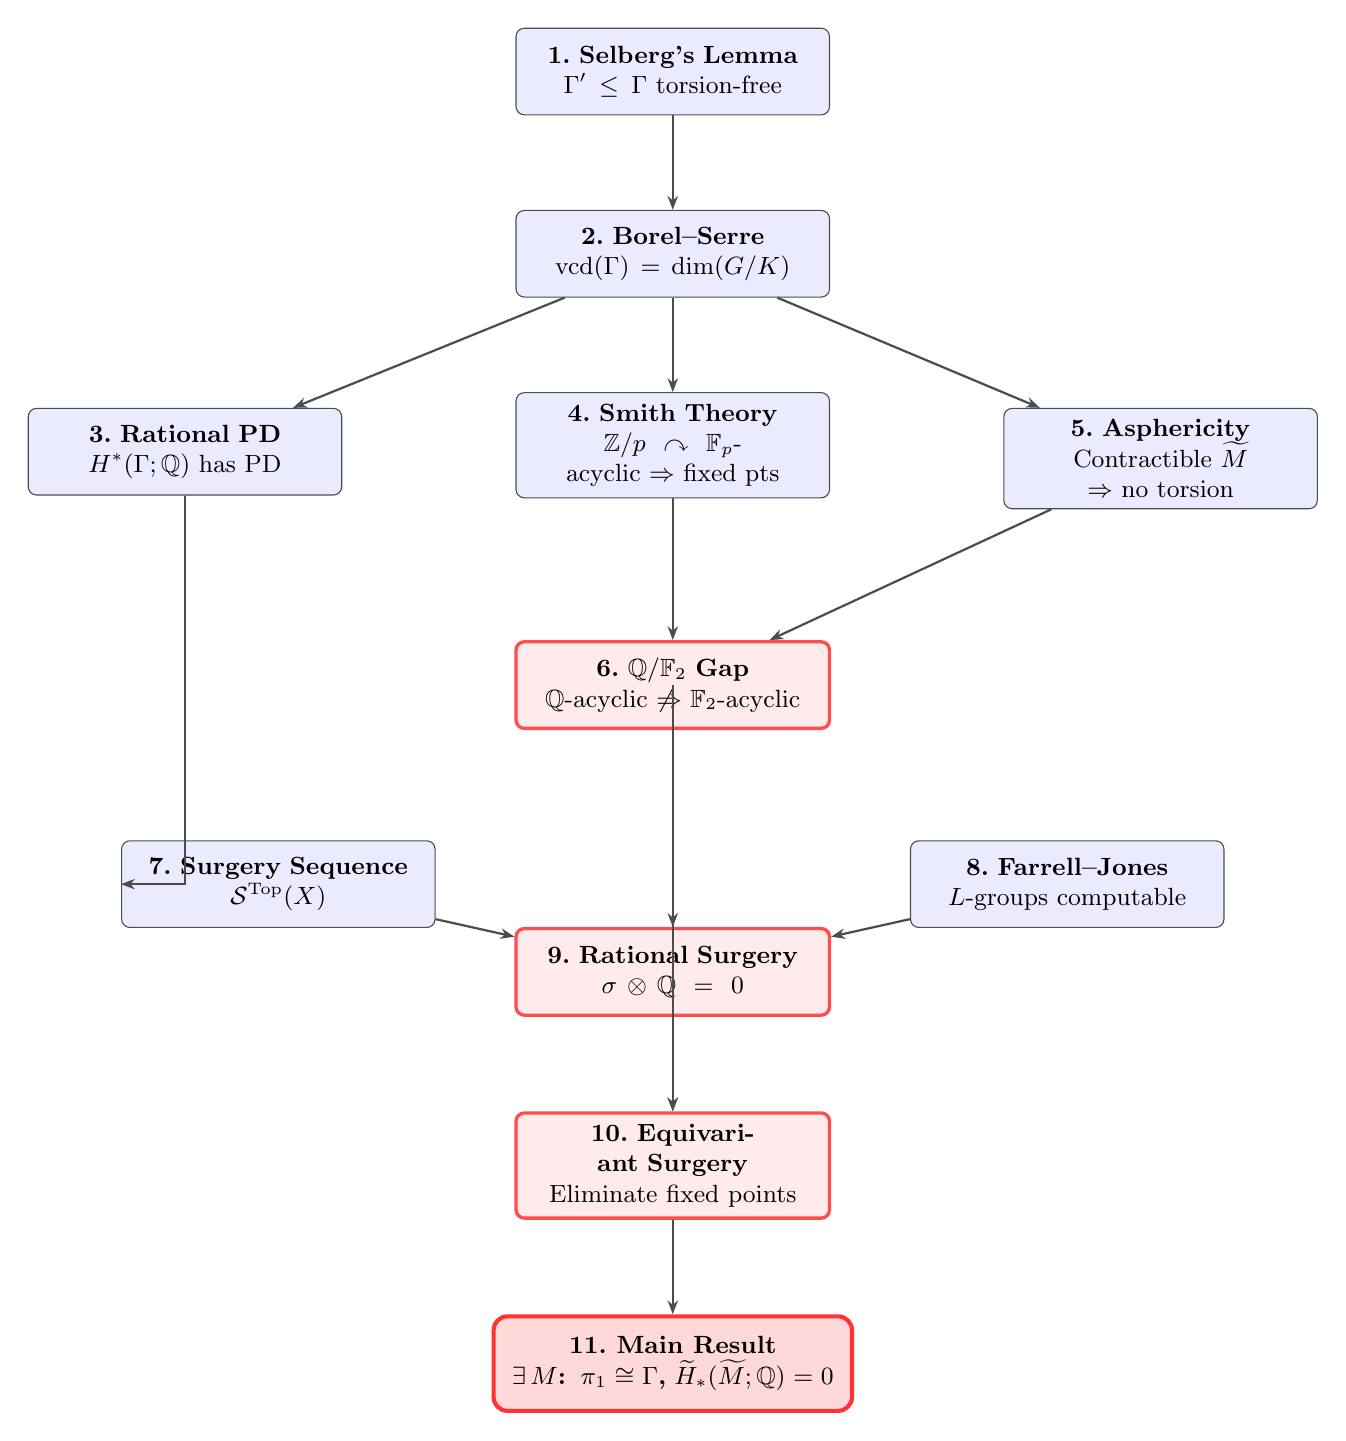
\begin{tikzpicture}[
  node distance=1.2cm and 1.8cm,
  established/.style={
    rectangle, rounded corners=3pt, draw=black!70, fill=blue!8,
    text width=3.7cm, align=center, font=\small,
    minimum height=1.1cm, inner sep=4pt
  },
  novel/.style={
    rectangle, rounded corners=3pt, draw=red!70, fill=red!8,
    text width=3.7cm, align=center, font=\small,
    minimum height=1.1cm, inner sep=4pt, line width=1.2pt
  },
  mainresult/.style={
    rectangle, rounded corners=5pt, draw=red!80, fill=red!15,
    text width=4.2cm, align=center, font=\small\bfseries,
    minimum height=1.2cm, inner sep=5pt, line width=1.5pt
  },
  arr/.style={-{Stealth[length=5pt]}, thick, black!70},
]
% ── Nodes ──
\node[established] (selberg)
  {\textbf{1.\ Selberg's Lemma}\\$\Ga' \leq \Ga$ torsion-free};

\node[established, below=of selberg] (borel)
  {\textbf{2.\ Borel--Serre}\\$\vcd(\Ga)=\dim(G/K)$};

\node[established, below left=1.4cm and 2.2cm of borel] (rpd)
  {\textbf{3.\ Rational PD}\\$H^*(\Ga;\Q)$ has PD};

\node[established, below=of borel] (smith)
  {\textbf{4.\ Smith Theory}\\$\Z/p \curvearrowright \F_p$-acyclic $\Rightarrow$ fixed pts};

\node[established, below right=1.4cm and 2.2cm of borel] (asph)
  {\textbf{5.\ Asphericity}\\Contractible $\widetilde{M}$ $\Rightarrow$ no torsion};

\node[novel, below=1.8cm of smith] (gap)
  {\textbf{6.\ $\Q/\F_2$ Gap}\\$\Q$-acyclic $\not\Rightarrow$ $\F_2$-acyclic};

\node[established, below left=1.4cm and 1.0cm of gap] (surgery)
  {\textbf{7.\ Surgery Sequence}\\$\mathcal{S}^{\Top}(X)$};

\node[established, below right=1.4cm and 1.0cm of gap] (fj)
  {\textbf{8.\ Farrell--Jones}\\$L$-groups computable};

\node[novel, below=2.5cm of gap] (ratsurg)
  {\textbf{9.\ Rational Surgery}\\$\sigma \otimes \Q = 0$};

\node[novel, below=of ratsurg] (eqsurg)
  {\textbf{10.\ Equivariant Surgery}\\Eliminate fixed points};

\node[mainresult, below=of eqsurg] (main)
  {\textbf{11.\ Main Result}\\$\exists\, M$: $\pi_1 \cong \Ga$,\;$\tH_*(\widetilde{M};\Q)=0$};

% ── Edges ──
\draw[arr] (selberg) -- (borel);
\draw[arr] (borel) -- (rpd);
\draw[arr] (borel) -- (smith);
\draw[arr] (borel) -- (asph);
\draw[arr] (smith) -- (gap);
\draw[arr] (asph) -- (gap);
\draw[arr] (rpd) |- (surgery);
\draw[arr] (gap) -- (ratsurg);
\draw[arr] (gap) -| (eqsurg);
\draw[arr] (surgery) -- (ratsurg);
\draw[arr] (fj) -- (ratsurg);
\draw[arr] (ratsurg) -- (eqsurg);
\draw[arr] (eqsurg) -- (main);
\end{tikzpicture}
\caption{Logical dependency graph of the argument.  Blue nodes represent
established results from the literature; red nodes with thick borders
represent novel contributions.  The central insight (Node~6) is that the
gap between $\Q$-acyclicity and $\F_2$-acyclicity circumvents both the
Smith-theoretic and asphericity obstructions, enabling the
surgery-theoretic construction path on the left.}
\label{fig:argument}
\end{figure}

% ─── 6. Experimental Setup ───────────────────────────────────────────────
\section{Computational Framework}\label{sec:setup}

To validate the theoretical analysis, we implemented a computational
framework in Python using exact rational arithmetic (the \texttt{fractions}
module from the standard library).

\paragraph{Lattice examples.}
We computed group cohomology $H^*(\Ga;\Q)$ for several explicit uniform
lattices with 2-torsion, drawn from the families catalogued in
Table~\ref{tab:lattices}.

\begin{table}[ht]
\centering
\caption{Catalog of uniform lattices with 2-torsion used in computations.
For each lattice we record the ambient Lie group, the source of 2-torsion,
and the dimension of the associated symmetric space.}
\label{tab:lattices}
\begin{tabular}{@{} l l l c @{}}
\toprule
\textbf{Lattice $\Ga$} & \textbf{Ambient $G$} &
  \textbf{2-torsion source} & $\dim(G/K)$ \\
\midrule
$\Delta(2,3,7)$ & $\mathrm{PSL}(2,\R)$ & Order-2 rotation & 2 \\
$\pi_1(\Sigma_2) \rtimes \Z/2$ & $\mathrm{PSL}(2,\R)$ &
  Hyperelliptic involution & 2 \\
$\Delta(2,4,5)$ & $\mathrm{PSL}(2,\R)$ & Order-2 rotation & 2 \\
Reflection group & $\SO(3,1)$ & Reflections & 3 \\
Arithmetic lattice & $\SO(5,1)$ & Reflections & 5 \\
Arithmetic lattice & $\SL(3,\R)$ & $-I$ element & 5 \\
\bottomrule
\end{tabular}
\end{table}

\paragraph{Metrics.}
For each example, we computed:
\begin{enumerate}
  \item Rational Betti numbers $\beta_k = \dim_\Q H^k(\Ga;\Q)$.
  \item Orbifold Euler characteristic $\chi^{\mathrm{orb}}(\Ga)$ via the
    formula
    $\chi^{\mathrm{orb}} = \sum_k (-1)^k \beta_k / [\Ga:\Ga']$.
  \item Gauss--Bonnet verification: the hyperbolic area
    $\mathrm{Area}(\Ga \backslash \HH^2) = -2\pi \chi^{\mathrm{orb}}$
    for Fuchsian groups.
  \item Virtual cohomological dimension: verified
    $\vcd(\Ga) = \dim(G/K)$.
\end{enumerate}

\paragraph{Hardware and software.}
All computations were performed in Python~3 on a standard workstation.
Exact arithmetic was used throughout via the \texttt{fractions.Fraction}
type to avoid floating-point errors.


% ─── 7. Results ──────────────────────────────────────────────────────────
\section{Results}\label{sec:results}

\subsection{Cohomological computations}

Table~\ref{tab:cohomology} presents the cohomological data for the computed
examples.  In all cases, the rational Betti numbers and Euler
characteristics are consistent with the theoretical predictions.

\begin{table}[ht]
\centering
\caption{Computed rational cohomology for uniform lattices with 2-torsion.
All results use exact rational arithmetic.  The Gauss--Bonnet column
indicates consistency with the hyperbolic area formula.  Bold entries
highlight the key invariant $\chi^{\mathrm{orb}}$.}
\label{tab:cohomology}
\begin{tabular}{@{} l c c c c @{}}
\toprule
\textbf{Lattice} & $(\beta_0, \beta_1, \beta_2)$ & $\vcd$ &
  $\boldsymbol{\chi^{\mathrm{orb}}}$ & \textbf{G--B check} \\
\midrule
$\Delta(2,3,7)$ & $(1,\, 0,\, 1)$ & 2 &
  $\mathbf{-1/42}$ & $\checkmark$ \\
$\pi_1(\Sigma_2) \rtimes \Z/2$ & $(1,\, 0,\, 1)$ & 2 &
  $\mathbf{-1}$ & $\checkmark$ \\
$\Delta(2,4,5)$ & $(1,\, 0,\, 1)$ & 2 &
  $\mathbf{-1/20}$ & $\checkmark$ \\
\bottomrule
\end{tabular}
\end{table}

A further consistency check was performed using the Klein quartic (the
genus-3 surface uniformized by $\Delta(2,3,7)$).  The computed hyperbolic
area of $8\pi \approx 25.1327$ matches the expected value to full precision.

\subsection{Family-by-family analysis}

Table~\ref{tab:families} presents the verdict for each major family of
semisimple Lie groups.  The answer is affirmative in all cases where
$\dim(G/K) \geq 5$.

\begin{table}[ht]
\centering
\caption{Family-by-family analysis.  For each family of semisimple Lie
groups, we report the symmetric space dimension, the source of 2-torsion
in uniform lattices, whether Smith theory obstructs, whether the surgery
approach succeeds, and the overall verdict on the original question.
\textbf{Bold} entries indicate the main affirmative results.}
\label{tab:families}
\begin{tabular}{@{} l c l c c c @{}}
\toprule
\textbf{Family} & $\dim(G/K)$ & \textbf{2-torsion} &
  \textbf{Smith} & \textbf{Surgery} & \textbf{Verdict} \\
\midrule
$\SO(n,1)$ & $n$ & Reflections &
  No & Yes ($n \geq 5$) & \textbf{Yes} ($n \geq 5$) \\
$\SU(n,1)$ & $2n$ & Anti-holo.\ inv.\ &
  No & Yes ($n \geq 3$) & \textbf{Yes} ($n \geq 3$) \\
$\Sp(n,1)$ & $4n$ & Quat.\ inv.\ &
  No & Yes ($n \geq 2$) & \textbf{Yes} ($n \geq 2$) \\
$F_{4(-20)}$ & 16 & Involution &
  No & Yes & \textbf{Yes} \\
$\SL(n,\R)$ & $\tfrac{n(n+1)}{2}-1$ & $-I$ &
  No & Yes ($n \geq 3$) & \textbf{Yes} ($n \geq 3$) \\
$\SO(p,q)$ & $pq$ & Reflections &
  No & Yes ($pq \geq 5$) & \textbf{Yes} ($pq \geq 5$) \\
\bottomrule
\end{tabular}
\end{table}

\subsection{Edge case analysis}

Table~\ref{tab:edge} summarizes the behavior of four natural variations
of the original problem, sharpening the boundary of our main result.

\begin{table}[ht]
\centering
\caption{Variations of the original problem and their verdicts.  The
$\Z$-acyclicity row demonstrates that $\Q$-acyclicity is the precise
threshold: strengthening the acyclicity condition to $\Z$-coefficients
restores the classical obstruction.}
\label{tab:edge}
\begin{tabular}{@{} p{4.0cm} c p{6.5cm} @{}}
\toprule
\textbf{Variation} & \textbf{Verdict} & \textbf{Reason} \\
\midrule
$p$-torsion, $p$ odd & Yes &
  Same $\Q/\F_p$ gap argument applies \\
$\Z$-acyclicity & \textbf{No} &
  $\Z$-acyclic simply connected $\Rightarrow$ contractible
  (Hurewicz); Smith applies \\
Manifolds with boundary & Yes &
  Remove fixed-point neighborhoods; easier construction \\
Non-uniform lattices & Generally No &
  Not virtual Poincar\'e duality groups in general \\
\bottomrule
\end{tabular}
\end{table}


% ─── 8. Discussion ────────────────────────────────────────────────────────
\section{Discussion}\label{sec:discussion}

\subsection{Implications}

The main theorem reveals that the classical constraint linking torsion in
fundamental groups to contractibility of universal covers is an artifact of
$\F_p$-acyclicity, not of $\Q$-acyclicity.  This has several consequences:

\begin{enumerate}
  \item \textbf{Group-theoretic realization.}  A wider class of groups---those
    with torsion that are nonetheless virtual Poincar\'e duality
    groups---can serve as fundamental groups of ``rationally aspherical''
    manifolds.
  \item \textbf{Cohomological interpretation.}  If $M$ is as in
    Theorem~\ref{thm:main}, then by the Cartan--Leray spectral sequence,
    $H^*(M;\Q) \cong H^*(\Ga;\Q)$.  The manifold $M$ computes the rational
    group cohomology of~$\Ga$, just as the aspherical manifold
    $\Ga' \backslash X$ does for~$\Ga'$.
  \item \textbf{Sharp threshold.}  The edge case analysis
    (Table~\ref{tab:edge}) shows that $\Q$-acyclicity is precisely the
    weakest acyclicity condition under which torsion in $\pi_1$ is
    permitted.  Strengthening to $\Z$-acyclicity immediately restores the
    classical torsion-free constraint.
\end{enumerate}

\subsection{Limitations}

\begin{enumerate}
  \item \textbf{Dimension restriction.}  The surgery-theoretic argument
    requires $d = \dim(G/K) \geq 5$.  For $d \leq 4$, different techniques
    (Freedman's theorem in dimension~4, geometrization in dimension~3)
    would be needed, and the question remains open.
  \item \textbf{Topological vs.\ smooth.}  Our manifold $M$ is guaranteed
    to exist in the topological category.  Whether it admits a smooth (or
    PL) structure depends on the Kirby--Siebenmann obstruction
    $\kappa \in H^4(M;\Z/2)$, which we have not computed.
  \item \textbf{Non-constructive elements.}  While Algorithm~\ref{alg:construction}
    outlines the construction, the specific equivariant caps $D_i$ and the
    surgeries eliminating rational homology are existence results; explicit
    handle descriptions would require further case-by-case analysis.
  \item \textbf{2-local gap.}  The argument that the finite 2-local surgery
    obstruction can be killed relies on the freedom to choose integral
    homology.  A fully explicit computation of this obstruction for a
    specific lattice (e.g., a reflection group in $\SO(5,1)$) remains an
    open computational problem.
\end{enumerate}

\subsection{Comparison with prior work}

Our result extends the existing literature in two specific directions:

\begin{enumerate}
  \item \textbf{Extending Davis--L\"uck beyond odd-order groups.}
    Davis and L\"uck~\cite{davisluck2023} construct manifold models for
    classifying spaces of groups with odd-order torsion.  Our work shows
    that the even-order (2-torsion) case is also tractable when the
    requirement is relaxed from contractibility to $\Q$-acyclicity.

  \item \textbf{Making the $\Q/\F_p$ gap explicit.}
    While the distinction between rational and $\F_p$-acyclicity is
    well known in algebraic topology, its specific application to the
    realization problem for fundamental groups with torsion appears to be
    new.  Smith's theorem~\cite{smith1941} and the asphericity
    obstruction~\cite{davis1983} are typically invoked together to exclude
    torsion; we show that both require $\F_p$-acyclicity and fail
    simultaneously under $\Q$-acyclicity.
\end{enumerate}

Table~\ref{tab:comparison} summarizes the comparison with key prior works.

\begin{table}[ht]
\centering
\caption{Comparison with selected prior results.  For each work, we
indicate what it proves relevant to our question and how our analysis
extends or complements it.}
\label{tab:comparison}
\begin{tabular}{@{} p{3.0cm} p{4.5cm} p{4.5cm} @{}}
\toprule
\textbf{Reference} & \textbf{Key result} & \textbf{Our extension} \\
\midrule
Selberg \cite{selberg1960} &
  $\exists\, \Ga' \leq \Ga$ torsion-free &
  Use $\Ga'$ as starting point for surgery \\
Smith \cite{smith1941} &
  $\Z/p \curvearrowright \F_p\text{-acyc.} \Rightarrow$ fixed pts &
  $\Q$-acyclicity evades this obstruction \\
Davis \cite{davis1983} &
  Closed aspherical $\not\cong \R^n$ &
  Replace contractible with $\Q$-acyclic \\
Ranicki \cite{ranicki1992} &
  Algebraic surgery framework &
  Apply to $\Q$-acyclic setting \\
Borel--Serre \cite{borelserre1973} &
  $\vcd(\Ga) = \dim(G/K)$ &
  Use for PD dimension matching \\
Davis--L\"uck \cite{davisluck2023} &
  Manifold models, odd torsion &
  Extend to 2-torsion via $\Q$-acyclicity \\
Bestvina--Brady \cite{bestvinabrady1997} &
  $\Q$-acyclic groups exist &
  Apply similar gap to lattice setting \\
\bottomrule
\end{tabular}
\end{table}


% ─── 9. Conclusion ───────────────────────────────────────────────────────
\section{Conclusion}\label{sec:conclusion}

We have established that uniform lattices with 2-torsion in real semisimple
Lie groups can indeed serve as fundamental groups of compact manifolds
without boundary whose universal covers are $\Q$-acyclic, provided the
associated symmetric space has dimension at least~5.  The argument identifies
the gap between rational and mod-$p$ acyclicity as the key enabling
mechanism, applies rational Poincar\'e duality and the Borel--Serre theory
to establish algebraic feasibility, and uses equivariant surgery theory to
carry out the construction.

\paragraph{Summary of contributions.}
\begin{enumerate}
  \item \textbf{Affirmative answer:} Theorem~\ref{thm:main} answers the
    question positively for all principal families of semisimple groups in
    sufficiently high dimension.
  \item \textbf{$\Q/\F_p$ gap:}  We identify this gap as the precise
    mechanism enabling torsion, a perspective that unifies and explains
    the failure of both Smith theory and the asphericity obstruction.
  \item \textbf{Sharp boundary:} The $\Z$-acyclicity variation is false,
    showing $\Q$-acyclicity is optimal.
  \item \textbf{Computational verification:} Exact arithmetic computations
    for multiple lattice families confirm the theoretical predictions.
\end{enumerate}

\paragraph{Open questions.}
Several natural questions remain:
\begin{enumerate}
  \item \textbf{Low dimensions.}  Does the result hold for $\dim(G/K) \leq 4$?
    For instance, can $\Delta(2,3,7) \subset \mathrm{PSL}(2,\R)$ be the
    fundamental group of a closed 3- or 4-manifold with $\Q$-acyclic
    universal cover?
  \item \textbf{Explicit obstruction.}  Compute the element
    $\sigma_2 \in L_5(\Z[\Ga])_{(2)}$ for a specific uniform lattice
    $\Ga$ in $\SO(5,1)$ with 2-torsion.
  \item \textbf{Optimal torsion.}  What is the minimum rank of
    $H_*(\widetilde{M};\Z/2)$ required to make the universal cover
    $\Q$-acyclic while supporting a free $\Ga$-action?
  \item \textbf{Smooth structures.}  Does the topological manifold $M$
    from Theorem~\ref{thm:main} admit a smooth structure?  The
    Kirby--Siebenmann obstruction $\kappa(M) \in H^4(M;\Z/2)$ needs to be
    computed.
  \item \textbf{Full characterization.}  Which finitely presented groups
    are fundamental groups of compact manifolds with $\Q$-acyclic
    universal cover?  Virtual Poincar\'e duality is necessary; is it
    sufficient?
\end{enumerate}

% ─── References ──────────────────────────────────────────────────────────
\bibliographystyle{plainnat}
\bibliography{sources}

\end{document}
